\section{Ćwiczenia 9: 4-V-2017}
\subsection{Zadania domowe A}
\paragraph{A1} Rozważmy łańcuch Markowa opisujący zabawę Orłosia i Resztki, z poprzedniego zestawu zadań domowych. Czy łańcuch jest nieprzywiedlny? Wyznacz okres każdego stanu tego łańcucha.

\begin{multicols}{2}[Łańcuch Orłosia i Resztki:]
\begin{table}[H]
\caption*{Stany:}
\centering
\begin{tabular}{cccc}
 & \multicolumn{3}{l}{Orłoś} \\
\multirow{3}{*}{Resztka} & \multicolumn{1}{l|}{} & \multicolumn{1}{l|}{N} & S \\ \cline{2-4} 
 & \multicolumn{1}{l|}{N} & \multicolumn{1}{l|}{\textbf{NN}} & \textbf{SN} \\ \cline{2-4} 
 & \multicolumn{1}{l|}{S} & \multicolumn{1}{l|}{\textbf{NS}} & \textbf{SS}
\end{tabular}
\end{table}
$$\mathbb{A}=\begin{bmatrix}
0&\frac{1}{2}&\frac{1}{2}&0\\
\frac{1}{2}&0&0&\frac{1}{2}\\
\frac{1}{2}&0&0&\frac{1}{2}\\
0&\frac{1}{2}&\frac{1}{2}&0
\end{bmatrix}$$
\begin{figure}[H]
\centering
\begin{tikzpicture}[shorten >=1pt, auto, node distance=3cm, ultra thick,main node/.style={circle,draw,minimum size=.4cm,inner sep=0pt}]
\begin{scope}[every node/.style={font=\sffamily\large\bfseries}]
%\node (v0) at (-2,2) {START};
\node [main node](v1) at (0,0) {\textbf{NN}};
\node [main node](v2) at (0,3) {\textbf{NS}};
\node [main node](v3) at (4,0) {\textbf{SN}};
\node [main node](v4) at (4,3) {\textbf{SS}};
\end{scope}
\path 
%	(v0) edge [->] (v1)
	(v1) edge [->,bend left] node {$\sfrac{1}{2}$} (v2)
         edge [->,bend left] node {$\sfrac{1}{2}$} (v3)
    (v2) edge [->,bend left] node {$\sfrac{1}{2}$} (v1)
         edge [->,bend left] node {$\sfrac{1}{2}$} (v4)
    (v3) edge [->,bend left] node {$\sfrac{1}{2}$} (v1)
         edge [->,bend left] node {$\sfrac{1}{2}$} (v4)
    (v4) edge [->,bend left] node {$\sfrac{1}{2}$} (v3)
         edge [->,bend left] node {$\sfrac{1}{2}$} (v2)
    ;
\end{tikzpicture}
\end{figure}
\end{multicols}
Przedstawiony Łańcuch jest nieprzywiedlny, gdyż (zgodnie z definicją: \ref{def:NieprzywiedlnoscLM} na stronie \pageref{def:NieprzywiedlnoscLM}) z każdego stanu prawdopodobieństwo ,,przejścia'' wynosi albo $\frac{1}{2}$ albo $\frac{1}{4}$ $\Rightarrow$ Łańcuch jest nieprzywiedlny.

Zgodnie z definicją (\ref{def:OkresStanuLM}, na stronie \pageref{def:OkresStanuLM}) możliwe czasy powrotów są równe: $2, 4, 6, ...$ a największy wspólny podzielnik (tych liczb) jest równy $2$. Więc (zgodnie z definicją: \ref{def:OkresLM}, na stronie \pageref{def:OkresLM}) $\mathsf{okr}=2$.

\paragraph{A2} Rozważmy łańcuch Markowa opisujący zachowanie żaby nad strumieniem, z poprzedniego zestawu zadań domowych. Wyznacz wszystkie rozkłady stacjonarne tego łańcucha.

\begin{multicols}{2}[Diagram stanów oraz macierz przejścia dla ,,żaby'']
\begin{figure}[H]
\centering
\begin{tikzpicture}[shorten >=1pt, auto, node distance=3cm, ultra thick,main node/.style={circle,draw,minimum size=.4cm,inner sep=0pt}]
\begin{scope}[every node/.style={font=\sffamily\large\bfseries}]
\node [main node](v1) at (0,0) {1};
\node [main node](v2) at (2,0) {2};
\end{scope}
\path 
	(v1) edge [->,bend left] node {$\sfrac{1}{3}$} (v2)
    	 edge [loop above]   node {$\sfrac{2}{3}$} (v1)
    (v2) edge [->,bend left] node {$\sfrac{1}{3}$} (v1)
    	 edge [loop above]   node {$\sfrac{2}{3}$} (v2)
         ;
\end{tikzpicture}
\end{figure}

$$\mathbb{P}=\begin{bmatrix}
\sfrac{2}{3}&\sfrac{1}{3}\\
\sfrac{1}{3}&\sfrac{2}{3}
\end{bmatrix}$$
\end{multicols}

\begin{align*}
&\bar{\pi}\mathbb{P}=\bar{\pi}\\
&\left[\pi _1, \pi _2\right]\begin{bmatrix}
\sfrac{2}{3}&\sfrac{1}{3}\\
\sfrac{1}{3}&\sfrac{2}{3}
\end{bmatrix} = \left[\pi _1, \pi _2\right]\\
&\left\{\begin{matrix}
\frac{2}{3}\pi _1 + \frac{1}{3}\pi _2 &= \pi _1\\
\frac{1}{3}\pi _1 + \frac{2}{3}\pi _2 &= \pi _2
\end{matrix}\right.\Leftrightarrow \left\{\begin{matrix}
\frac{1}{3}\pi _2 &= \pi _1-\frac{2}{3}\pi _1\\
\frac{1}{3}\pi _1+ \frac{2}{3}\pi _2 &= \pi _2
\end{matrix}\right.\Leftrightarrow \left\{\begin{matrix}
\pi _2 &= 3\pi _1-2\pi _1\\
\frac{1}{3}\pi _1 + \frac{2}{3}\pi _2 &= \pi _2
\end{matrix}\right.\\
&\pi _2 = \pi _1\\
&2\pi _1 = 1 \Leftrightarrow \pi _1 = \frac{1}{2}
\end{align*} 
Rozkład stacjonarny ma postać: $\left[\frac{1}{2}, \frac{1}{2}\right]$

\paragraph{A3} Wyznacz przynajmniej jeden rozkład stacjonarny dla łańcucha Markowa o podanej macierzy przejścia
\begin{enumerate}[label=\alph*)]
\item 
$$\begin{bmatrix}
1&0&0&0\\
0&\frac{1}{4}&\frac{3}{4}&0\\
0&\frac{1}{4}&\frac{3}{4}&0\\
\frac{1}{4}&\frac{1}{4}&\frac{1}{4}&\frac{1}{4}
\end{bmatrix}$$
\begin{align*}
&\bar{\pi}\mathbb{P}=\bar{\pi}\\
&\left[\pi _1, \pi _2,\pi _3,\pi _4\right]\begin{bmatrix}
1&0&0&0\\
0&\frac{1}{4}&\frac{3}{4}&0\\
0&\frac{1}{4}&\frac{3}{4}&0\\
\frac{1}{4}&\frac{1}{4}&\frac{1}{4}&\frac{1}{4}
\end{bmatrix}=\left[\pi _1, \pi _2,\pi _3,\pi _4\right]\\
&\left\{\begin{matrix}
\pi _1+\frac{1}{4}\pi _4 & = \pi _1\\
\frac{1}{4}\pi _2+\frac{1}{4}\pi _3 &= \pi _2\\
\frac{3}{4}\pi _2\frac{3}{4}\pi _3 &= \pi _3\\
\frac{1}{4}\pi _4 &= \pi _4
\end{matrix}\right.\Leftrightarrow \left\{\begin{matrix}
\pi _1 & = \pi _1\\
\frac{1}{4}\pi _2+\frac{1}{4}\pi _3 &= \pi _2\\
\frac{3}{4}\pi _2\frac{3}{4}\pi _3 &= \pi _3\\
\pi _4 &= 0
\end{matrix}\right.\Leftrightarrow \left\{\begin{matrix}
\pi _1 & = \pi _1\\
\pi _3 &= 3\pi _2\\
3\pi _2 &= \pi _3\\
\pi _4 &= 0
\end{matrix}\right.\Leftrightarrow \left\{\begin{matrix}
\pi _1 & = 0\\
\pi _2 &= \frac{1}{3}\pi _3\\
\pi _3 &= 3\pi _2\\
\pi _4 &= 0
\end{matrix}\right.\\
\end{align*}
Rozkład stacjonarny ma postać: $\left[0, \frac{1}{4}, \frac{3}{4}, 0\right]$

\item 
$$\begin{bmatrix}
\frac{1}{4}&\frac{1}{4}&\frac{1}{4}&\frac{1}{4}\\
0&0&\frac{3}{4}&\frac{1}{4}\\
0&0&0&1\\
0&0&0&1
\end{bmatrix}$$
\begin{align*}
&\bar{\pi}\mathbb{P}=\bar{\pi}\\
&\left[\pi _1, \pi _2,\pi _3,\pi _4\right]\begin{bmatrix}
\frac{1}{4}&\frac{1}{4}&\frac{1}{4}&\frac{1}{4}\\
0&0&\frac{3}{4}&\frac{1}{4}\\
0&0&0&1\\
0&0&0&1
\end{bmatrix} = \left[\pi _1, \pi _2,\pi _3,\pi _4\right]\\
&\left\{\begin{matrix}
\frac{1}{4}\pi _1 &= \pi _1\\
\frac{1}{4}\pi _1 &= \pi _2\\
\frac{1}{4}\pi _1 +\frac{3}{4} \pi _2&= \pi _3\\
\frac{1}{4}\pi _1 +\frac{1}{4} \pi _2+\pi _3 + \pi _4&= \pi _4\\
\end{matrix}\right.\Leftrightarrow \left\{\begin{matrix}
\pi _1 &= 0\\
\pi _2 &= 0\\
\pi _3&= 0\\
\pi _4&= \pi _4\\
\end{matrix}\right. \Leftrightarrow \left\{\begin{matrix}
\pi _1 = \pi _2=\pi _3 &= 0\\
\pi _4&= 1\\
\end{matrix}\right.
\end{align*}
Rozkład stacjonarny ma postać: $\left[0, 0, 0, 1\right]$

\item 
$$\begin{bmatrix}
0&\frac{1}{2}&0&\frac{1}{2}\\
\frac{1}{3}&0&\frac{1}{3}&\frac{1}{3}\\
0&\frac{1}{2}&0&\frac{1}{2}\\
\frac{1}{3}&\frac{1}{3}&\frac{1}{3}&0
\end{bmatrix}$$
\begin{align*}
&\bar{\pi}\mathbb{P}=\bar{\pi}\\
&\left[\pi _1, \pi _2,\pi _3,\pi _4\right]\begin{bmatrix}
0&\frac{1}{2}&0&\frac{1}{2}\\
\frac{1}{3}&0&\frac{1}{3}&\frac{1}{3}\\
0&\frac{1}{2}&0&\frac{1}{2}\\
\frac{1}{3}&\frac{1}{3}&\frac{1}{3}&0
\end{bmatrix} = \left[\pi _1, \pi _2,\pi _3,\pi _4\right]\\
& \left\{\begin{matrix}
\frac{1}{3} \pi _2 + \frac{1}{3} \pi _4 &= \pi _1\\
\frac{1}{2} \pi _1 + \frac{1}{2} \pi _3 + \frac{1}{3} \pi _4 &= \pi _2\\
\frac{1}{3} \pi _2 + \frac{1}{3} \pi _4 &= \pi _3\\
\frac{1}{2} \pi _1 + \frac{1}{3} \pi _2 + \frac{1}{2} \pi _3 &= \pi _4
\end{matrix}\right. \Leftrightarrow \left\{\begin{matrix}
\pi _1  &= \pi _3\\
\pi _1 + \frac{1}{3} \pi _4 &= \pi _2\\
\frac{1}{3} \pi _2 + \frac{1}{3} \pi _4 &= \pi _3\\
\pi _1 + \frac{1}{3} \pi _2 &= \pi _4
\end{matrix}\right.\Leftrightarrow \left\{\begin{matrix}
\pi _1  &= \pi _3\\
\pi _1 + \frac{1}{3} \pi _4 &= \pi _2\\
\frac{1}{3} \pi _2 + \frac{1}{3} \pi _4 &= \pi _3\\
\pi _1 + \frac{1}{3}\left(\pi _1 + \frac{1}{3} \pi _4\right) &= \pi _4
\end{matrix}\right.\\
& \Leftrightarrow \left\{\begin{matrix}
\pi _1  &= \pi _3\\
\pi _1 + \frac{1}{3} \pi _4 &= \pi _2\\
\frac{1}{3} \pi _2 + \frac{1}{3} \pi _4 &= \pi _3\\
\pi _4 &= \frac{3}{2}\pi _1
\end{matrix}\right. \Leftrightarrow \left\{\begin{matrix}
\pi _1  &= \pi _3\\
\pi _2 & = \frac{3}{2}\pi _1\\
\frac{1}{3} \pi _2 + \frac{1}{3} \pi _4 &= \pi _3\\
\pi _4 &= \frac{3}{2}\pi _1
\end{matrix}\right.\Leftrightarrow \left\{\begin{matrix}
\pi _1  &= \pi _3\\
\pi _2 & = \frac{3}{2}\pi _1\\
\pi _3 &= \pi _1\\
\pi _4 &= \frac{3}{2}\pi _1
\end{matrix}\right.\\
& x + \frac{3}{2}x+x+\frac{3}{2}x = 1\Leftrightarrow 5x = 1\Leftrightarrow x = \frac{1}{5} = 0.2
\end{align*}
Rozkład stacjonarny ma postać: $\left[\frac{1}{5}, \frac{3}{10}, \frac{1}{5}, \frac{3}{10}\right]$
\item 
$$\begin{bmatrix}
\frac{1}{3}&0&\frac{2}{3}&0&0\\
\frac{2}{3}&0&\frac{1}{3}&0&0\\
0&\frac{3}{4}&0&\frac{1}{4}&0\\
0&\frac{1}{2}&0&\frac{1}{4}&\frac{1}{4}\\
0&\frac{1}{2}&0&\frac{1}{2}&0
\end{bmatrix}$$
\begin{align*}
&\bar{\pi}\mathbb{P}=\bar{\pi}\\
&\left[\pi _1, \pi _2,\pi _3,\pi _4,\pi _5\right]\begin{bmatrix}
\frac{1}{3}&0&\frac{2}{3}&0&0\\
\frac{2}{3}&0&\frac{1}{3}&0&0\\
0&\frac{3}{4}&0&\frac{1}{4}&0\\
0&\frac{1}{2}&0&\frac{1}{4}&\frac{1}{4}\\
0&\frac{1}{2}&0&\frac{1}{2}&0
\end{bmatrix}=\left[\pi _1, \pi _2,\pi _3,\pi _4,\pi _5\right]\\
&\left\{\begin{matrix}
\frac{1}{3}\pi _1+\frac{2}{3}\pi _2 &= \pi _1\\
\frac{3}{4}\pi _3 + \frac{1}{2}\pi _4+\frac{1}{2}\pi _5 &= \pi _2\\
\frac{2}{3}\pi _1+\frac{1}{3}\pi _2 &= \pi _3\\
\frac{1}{4}\pi _3+\frac{1}{4}\pi _4+\frac{1}{2}\pi _5 &= \pi _4\\
\frac{1}{4}\pi _4 &= \pi _5
\end{matrix}\right.\Leftrightarrow \left\{\begin{matrix}
\pi _1 = \pi _2 = \pi _3\\
\pi _4 = \frac{2}{5} \pi _1\\
\pi _5 = \frac{1}{10} \pi _1
\end{matrix}\right.\\
& x+x+x+\frac{2}{5}x + \frac{1}{10} x = 1\Leftrightarrow \frac{7}{2}x=1 \Leftrightarrow x = \frac{2}{7}
\end{align*}
\end{enumerate}
Rozkład stacjonarny ma postać: $\left[\frac{2}{7}, \frac{2}{7}, \frac{2}{7}, \frac{4}{35}, \frac{1}{35}\right]$

\paragraph{A4} Na ćwiczeniach opisaliśmy dramatyczną sytuację spragnionego Bolka za pomocą łańcucha Markowa.
\begin{multicols}{2}[Przedstawienie \textbf{dramatycznej} sytuacji Bolka:]
\begin{figure}[H]
\centering
\begin{tikzpicture}[shorten >=1pt, auto, node distance=3cm, ultra thick,main node/.style={circle,draw,minimum size=.4cm,inner sep=0pt}]
\begin{scope}[every node/.style={font=\sffamily\large\bfseries}]
\node [main node](v0) at (0,0) {0};
\node [main node](v1) at (2,0) {1};
\node [main node](v2) at (4,0) {2};
\node [main node](v3) at (6,0) {3};
\end{scope}
\path 
	(v0) edge [loop above]   node {$1$} (v0)
    (v1) edge [->,bend left] node {$\sfrac{1}{2}$} (v0)
    	 edge [->,bend left] node {$\sfrac{1}{2}$} (v2)
    (v2) edge [->,bend left] node {$\sfrac{1}{2}$} (v1)
    	 edge [->,bend left] node {$\sfrac{1}{2}$} (v3)
    (v3) edge [loop above]   node {$1$} (v3)
         ;
\end{tikzpicture}
\end{figure}

$$\mathbb{P}=\begin{bmatrix}
1&0&0&0\\
\frac{1}{2}&0&\frac{1}{2}&0\\
0&\frac{1}{2}&0&\frac{1}{2}\\
0&0&0&1
\end{bmatrix}$$
\end{multicols}
\begin{enumerate}[label=\alph*)]
\item Czy łańcuch ten jest nieprzywiedlny? Czy jest okresowy?

\textbf{Nie}, nie jest to łańcuch nieprzywiedlny, gdyż ze stanów $0$ i $3$ nie można ,,przejść'' w żaden inny stan. 


Łańcuch nie jest okresowy, ale stany $1$ i $2$ posiadają okres 2.

\item Czy istnieje dla niego rozkład stacjonarny?
\begin{align*}
&\bar{\pi}\mathbb{P}=\bar{\pi}\\
&\left[\pi _1, \pi _2,\pi _3,\pi _4\right]\begin{bmatrix}
1&0&0&0\\
\frac{1}{2}&0&\frac{1}{2}&0\\
0&\frac{1}{2}&0&\frac{1}{2}\\
0&0&0&1
\end{bmatrix}=\left[\pi _1, \pi _2,\pi _3,\pi _4\right]\\
&\left\{\begin{matrix}
\pi _1 + \frac{1}{2} \pi _2 &= \pi _1\\
\frac{1}{2} \pi _3 &= \pi _2\\
\frac{1}{2} \pi _2 &= \pi _3\\
\frac{1}{2} \pi _3 + \pi _4 &= \pi _4
\end{matrix}\right. \rightarrow \left\{\begin{matrix}
\pi _1  &= \pi _1\\
\pi _2 = \pi _3 &= 0\\
\pi _4 &= \pi _4
\end{matrix}\right.\\
&\text{ równanie nie oznaczone? ale chyba jest: } \left[\frac{1}{3}, 0, 0, \frac{2}{3}\right]
\end{align*}
Ogólny wzór na rozkład stacjonarny: $\left[\pi _1, 0, 0, 1-\pi _1\right]$ gdzie $\pi _1 \in (0; 1)$
\end{enumerate}

\paragraph{A5} Rozważmy łańcuch Markowa z robaczkami z ostatniego zadania poprzednich ćwiczeń (model z 4 stanami, numery wierzchołków trójkąta nie są istotne).
\begin{multicols}{2}[Przedstawienie macierzy ,,robaczków'']
z  dokładnym rozłożeniem kolorów robaczków na trójkącie\\
$|S|=8$, (góra, lewo, prawo)\\ $S=\{ccc,zzz,czz,zzc,zcz,zcc,ccz,czc\}$
$$\mathbb{P}=\begin{bmatrix}
1&0&0&0&0&0&0&0\\
0&1&0&0&0&0&0&0\\
0&\frac{1}{4}&0&\frac{1}{4}&\frac{1}{4}&\frac{1}{4}&0&0\\
0&\frac{1}{4}&\frac{1}{4}&0&\frac{1}{4}&0&\frac{1}{4}&0\\
0&\frac{1}{4}&\frac{1}{4}&\frac{1}{4}&0&0&0&\frac{1}{4}\\
\frac{1}{4}&0&\frac{1}{4}&0&0&0&\frac{1}{4}&\frac{1}{4}\\
\frac{1}{4}&0&0&\frac{1}{4}&0&\frac{1}{4}&0&\frac{1}{4}\\
\frac{1}{4}&0&0&0&\frac{1}{4}&\frac{1}{4}&\frac{1}{4}&0
\end{bmatrix}$$

liczba robaczków w obu kolorach
$|S|=4$, $S=\{3c,3z,2c1z,2z1c\}$
$$\begin{bmatrix}
1&0&0&0\\
0&1&0&0\\
\frac{1}{4}&0&\frac{1}{2}&\frac{1}{4}\\
0&\frac{1}{4}&\frac{1}{4}&\frac{1}{2}
\end{bmatrix}$$
\end{multicols}
\begin{enumerate}[label=\alph*)]
\item Wyznacz przynajmniej trzy rozkłady stacjonarne tego łańcucha.

\begin{align*}
&\bar{\pi}\mathbb{P}=\bar{\pi}\\
&\left[\pi _1, \pi _2,\pi _3,\pi _4\right]\begin{bmatrix}
1&0&0&0\\
0&1&0&0\\
\frac{1}{4}&0&\frac{1}{2}&\frac{1}{4}\\
0&\frac{1}{4}&\frac{1}{4}&\frac{1}{2}
\end{bmatrix}=\left[\pi _1, \pi _2,\pi _3,\pi _4\right]\\
&\left\{\begin{matrix}
\pi _1 +\frac{1}{4}\pi _3 &= \pi _1\\
\pi _2 + \frac{1}{4}\pi _4 &= \pi _2\\
\frac{1}{2}\pi _3+\frac{1}{4}\pi _4 &= \pi _3\\
\frac{1}{4}\pi _3+\frac{1}{2}\pi _4 &= \pi _4
\end{matrix}\right.\rightarrow \left\{\begin{matrix}
\pi _1 &= \pi _1\\
\pi _2 &= \pi _2\\
\pi _3 = \pi _4 &= 0
\end{matrix}\right.
\end{align*}
Przykładowe rozkłady stacjonarne?
\begin{itemize}
\item $ \left[\frac{1}{3}, \frac{2}{3},0,0\right]$
\item $ \left[\frac{1}{4}, \frac{3}{4},0,0\right]$
\item $ \left[\frac{1}{5}, \frac{4}{5},0,0\right]$
\end{itemize}

\item Uzasadnij, że łańcuch jest odwracalny.
Zgodnie z definicją (\ref{def:OdwracalnoscLM}, na stronie \pageref{def:OdwracalnoscLM}) szukamy wektora $\bar{a}$ takiego, że $a_i\pi_{ij}=a_j\pi_{ji}$ 
\begin{figure}[H]
\centering
\begin{tikzpicture}[shorten >=1pt, auto, node distance=3cm, ultra thick,main node/.style={circle,draw,minimum size=.4cm,inner sep=0pt}]
\begin{scope}[every node/.style={font=\sffamily\large\bfseries}]
\node [main node,label=below:$1$](v0) at (0,0) {3c};
\node [main node,label=above:$2$](v1) at (4,4) {3z};
\node [main node,label=below:$3$](v2) at (4,0) {2c1z};
\node [main node,label=above:$4$](v3) at (0,4) {2z1c};
\end{scope}
\path 
	(v0) edge [loop left]   node {$1$} (v0)
    (v1) edge [loop right]   node {$1$} (v1)
    (v2) edge [->,bend left] node {$\sfrac{1}{4}$} (v0)
    	 edge [loop right] node {$\sfrac{1}{2}$} (v2)
         edge [->,bend left] node {$\sfrac{1}{4}$} (v3)
    (v3) edge [->,bend left] node {$\sfrac{1}{4}$} (v1)
    	 edge [->,bend left] node {$\sfrac{1}{4}$} (v2)
         edge [loop left] node {$\sfrac{1}{2}$} (v3)
         ;
\end{tikzpicture}
\caption*{Diagram stanów (może pomoże)}
\end{figure}
Tylko dla stanów 3 i 4 (2z1c i 2c1z) można wyliczyć wektor $\bar{a}$, a że $\pi _{3,4}=\pi _{4,3}=\frac{1}{4}$ to $a_3=a_4$ czyli na przykład: $\bar{a}=\left[0,0,1,1\right]$ 

\begin{align*}
a_i\pi _{i,j}=a_j\pi _{j,i}\\
\left\{\begin{matrix}
a_1*\pi _{1,2} &= a_2\pi _{2,1}\\
a_1*\pi _{1,3} &= a_3\pi _{3,1}\\
a_1*\pi _{1,4} &= a_4\pi _{4,1}\\
a_2*\pi _{2,1} &= a_1\pi _{1,2}\\
a_2*\pi _{2,3} &= a_3\pi _{3,2}\\
a_2*\pi _{2,4} &= a_4\pi _{4,2}\\
a_3*\pi _{3,1} &= a_1\pi _{1,3}\\
a_3*\pi _{3,2} &= a_2\pi _{2,3}\\
a_3*\pi _{3,4} &= a_4\pi _{4,3}\\
a_4*\pi _{4,1} &= a_1\pi _{1,3}\\
a_4*\pi _{4,2} &= a_2\pi _{2,3}\\
a_4*\pi _{4,3} &= a_3\pi _{3,3}
\end{matrix}\right.
\end{align*}
\todo[inline,color=red!20]{układ równań, sprawdzić}
\end{enumerate}

\paragraph{A6} Myszka Honoratka wędruje pomiędzy norką, spiżarnią i ciepłym miejscem przy kominku rzucając kostką co kwadrans. Jeśli siedzi w norce, a wypadnie szóstka, wędruje do spiżarni, Jeśli jest w spiżarni i wypadnie jedynka, dwójka lub trójka, to udaje się do kominka, a gdy siedzi przy kominku i wypadnie czwórka lub trójka, wraca do norki. W pozostałych przypadkach Honoratka siedzi cichutko na miejscu, które właśnie zajmuje. Wyznacz macierz przejścia dla łańcucha Markowa opisującego podróż Honoratki i oceń, czy łańcuch ten jest odwracalny.

Stany $S=\{N,S,K\}$ (Norka, Spiżarnia, Kominek) (założenie, że jest to sześcienne kostka)
$$\mathbb{P}=\begin{bmatrix}
\sfrac{5}{6}&\sfrac{1}{6}&0\\
0&\sfrac{1}{2}&\sfrac{1}{2}\\
\sfrac{1}{3}&0&\sfrac{2}{3}
\end{bmatrix}$$
\begin{figure}[H]
\centering
\begin{tikzpicture}[shorten >=1pt, auto, node distance=3cm, ultra thick,main node/.style={circle,draw,minimum size=.4cm,inner sep=0pt}]
\begin{scope}[every node/.style={font=\sffamily\large\bfseries}]
\node [main node,label=below:$1$](v1) at (2,0) {N};
\node [main node,label=below:$2$](v2) at (4,0) {S};
\node [main node,label=above:$3$](v3) at (3,2) {K};
\end{scope}
\path 
    (v1) edge [loop left] node {$\sfrac{5}{6}$} (v1)
    	 edge [->,bend right] node[below] {$\sfrac{1}{6}$} (v2)
    (v2) edge [loop right] node {$\sfrac{1}{2}$} (v2) 
    	 edge [->,bend right] node {$\sfrac{1}{2}$} (v3)
    (v3) edge [loop left]   node {$\frac{2}{3}$} (v3)
    	 edge [->,bend right] node {$\sfrac{1}{3}$} (v1)
         ;
\end{tikzpicture}
\end{figure}
Zgodnie z definicją (\ref{def:OdwracalnoscLM}, na stronie \pageref{def:OdwracalnoscLM}) szukamy wektora $\bar{a}$ takiego, że $a_i\pi_{ij}=a_j\pi_{ji}$, czyli:
\begin{align*}
&\bar{a}=\left\{\begin{matrix}
a_1\pi _{1,2} &= a_2\pi _{2,1}\\
a_2\pi _{2,3} &= a_3\pi _{3,2}\\
a_3\pi _{3,1} &= a_1\pi _{1,3}
\end{matrix}\right. \rightarrow \left\{\begin{matrix}
\sfrac{1}{6}\,a_1 &= \sfrac{1}{2}*\sfrac{1}{3}\,a_2\\
\sfrac{1}{2}\,a_2 &= \sfrac{1}{3}*\sfrac{1}{6}\,a_3\\
\sfrac{1}{3}\,a_3 &= \sfrac{1}{6}*\sfrac{1}{2}\,a_1
\end{matrix}\right. \rightarrow \left\{\begin{matrix}
\sfrac{1}{6}\,a_1 &= \sfrac{1}{6}\,a_2\\
\sfrac{1}{2}\,a_2 &= \sfrac{1}{18}\,a_3\\
\sfrac{1}{3}\,a_3 &= \sfrac{1}{12}\,a_1
\end{matrix}\right.\rightarrow \\
&\rightarrow \left\{\begin{matrix}
a_1 &= a_2\\
a_2 &= \sfrac{1}{9}\,a_3\\
a_3 &= \sfrac{1}{4}\,a_1
\end{matrix}\right.
\end{align*}
Otrzymujemy sprzeczność, gdyż  $a_1 = \frac{1}{9}a_3$ i równocześnie $\frac{1}{4}a_1 = a_3$\\
Więc \textbf{nie} jest to łańcuch odwracalny, gdyż spacerując po tym łańcuchu mamy ,,tendencję'' do ,,przemieszczania się'' w przeciwnym kierunku wskazówek zegara.

\paragraph{A7} Rozważmy łańcuch Markowa opisujący nieklasyczne błądzenie cząsteczki po ścieżce o 3 wierzchołkach, z poprzedniego zestawu zadań domowych.
\begin{multicols}{2}[Przedstawienie błądzenia cząsteczki wraz z macierzą:]
\begin{figure}[H]
\centering
\begin{tikzpicture}[shorten >=1pt, auto, node distance=3cm, ultra thick,main node/.style={circle,draw,minimum size=.4cm,inner sep=0pt}]
\begin{scope}[every node/.style={font=\sffamily\large\bfseries}]
\node [main node,label=below:$1$](v1) at (0,0) {\textbf{-1}};
\node [main node,label=below:$2$](v2) at (3,0) {\textbf{0}};
\node [main node,label=below:$3$](v3) at (6,0) {\textbf{1}};
\end{scope}
\path 
	(v1) edge [loop above] node {$\sfrac{1}{2}$} (v1)
         edge [->,bend left] node {$\sfrac{1}{2}$} (v2)
    (v2) edge [loop above] node {$\sfrac{1}{2}$} (v2)
         edge [->,bend left] node {$\sfrac{1}{4}$} (v1)
         edge [->,bend left] node {$\sfrac{1}{4}$} (v3)
    (v3) edge [loop above] node {$\sfrac{1}{2}$} (v3)
         edge [->,bend left] node {$\sfrac{1}{2}$} (v2)
    ;
\end{tikzpicture}
\caption*{Oznaczenia stanów pod wierzchołkami}
\end{figure}
$$\mathbb{P}=\begin{bmatrix}
\frac{1}{2}&\frac{1}{2}&0\\
\frac{1}{4}&\frac{1}{2}&\frac{1}{4}\\
0&\frac{1}{2}&\frac{1}{2}
\end{bmatrix}$$
\end{multicols}
\begin{enumerate}[label=\alph*)]
\item Sprawdź, że łańcuch ten jest nieprzywiedlny i nieokresowy.

Tak podany łańcuch jest nieprzywiedlny, gdyż dla każdej pary stanów $i,j$:
\begin{align*}
&\pi _{12}(1) = \frac{1}{2} &\pi _{13}(2) = \frac{1}{2}*\frac{1}{4}=\frac{1}{8}\\
&\pi _{21}(1) =\frac{1}{4} &\pi _{23}(1) =\frac{1}{4}\\
&\pi _{31}(2) =\frac{1}{2}*\frac{1}{4}=\frac{1}{8}&\pi _{32}(1) =\frac{1}{2}
\end{align*}
więc dla każdego stanu istnieje $t$ takie, że $\pi_{ij}(t)>0$.

Każdy wierzchołek posiada ,,pętle własną'' (którą ,,przechodzi'' z prawdopodobieństwem $\frac{1}{2}$) więc każdy stan ma okres 1 (definicja \ref{def:OkresStanuLM} na stronie \pageref{def:OkresStanuLM}). Dodatkowo z faktu, że łańcuch jest nieprzywiedlny (dowód wyżej), i z faktu na stronie \pageref{fac:OkresLM} to okres przedstawionego łańcucha wynosi $\mathsf{okr}(Ł)=1$.
\item Jakie rozkłady stacjonarne posiada?

\begin{align*}
&\bar{\pi}\mathbb{P}=\bar{\pi}\\
&\left[\pi _1, \pi _2,\pi _3\right]\begin{bmatrix}
\frac{1}{2}&\frac{1}{2}&0\\
\frac{1}{4}&\frac{1}{2}&\frac{1}{4}\\
0&\frac{1}{2}&\frac{1}{2}
\end{bmatrix}=\left[\pi _1, \pi _2,\pi _3\right]\\
&\left\{\begin{matrix}
\frac{1}{2}\pi _1 + \frac{1}{4}\pi _2&=\pi _1\\
\frac{1}{2}\pi _1+\frac{1}{2}\pi _2+\frac{1}{2}\pi _3&=\pi _2\\
\frac{1}{4}\pi _2+\frac{1}{2}\pi _3 &=\pi _3
\end{matrix}\right. \rightarrow \left\{\begin{matrix}
\pi _1 &=\frac{1}{2}\pi _2\\
\pi _2 &= 2\pi _1\\
\pi _3&= \pi _1
\end{matrix}\right.
&\pi _1 + \pi_2 + \pi _3 = 1\\
&\left\{\begin{matrix}
\pi _2 &= 2\pi _1\\
\pi _3&= \pi _1
\end{matrix}\right.\\
&\pi _1 + 2\pi _1 + \pi _1 = 1, \ \ \pi _1\in (0;1)\\
&\pi _1 = \frac{1}{4}\\
&\text{Rozkład stacjonarny }:\left[\frac{1}{4}, \frac{1}{2}, \frac{1}{4}\right]
\end{align*}

\item Jakie jest w przybliżeniu prawdopodobieństwo przejścia ze stanu -1 do stanu 0 w 2000 krokach? Błąd przybliżenia nie jest istotny.

Na podstawie twierdzenia o Ergodyczności (\ref{the:ergodycznoscLM2} na stronie \pageref{the:ergodycznoscLM2}) (dokładniej podpunkt 3) możemy ,,przybliżyć'' wartość prawdopodobieństwa przejścia ze stanu $-1$ do $0$ (stano oznaczone jako $1$ i $2$) w następujący sposób:
\begin{align*}
&\lim _{n\rightarrow \infty} \mathsf{Pr}_{a,b}=\pi _b\\
&\mathsf{Pr}_{1,2}(2000)\approx \pi _2\\
&\mathsf{Pr}_{1,2}(2000)\approx \frac{1}{2}
\end{align*}
\item Jakie jest w przybliżeniu prawdopodobieństwo, że po 2000 krokach cząsteczka znajdzie się w wierzchołku -1? Proszę zwrócić uwagę , że w przeciwieństwie do poprzedniego podpunktu, tu nic nie wiemy o rozkładzie początkowym.

Ponownie korzystając z twierdzenia o Ergodyczności (\ref{the:ergodycznoscLM2} na stronie \pageref{the:ergodycznoscLM2}) szukamy prawdopodobieństwo przejścia do stanu $-1$ z wszystkich pozostałych stanów, a więc:
\begin{align*}
&\lim _{n\rightarrow \infty} \mathsf{Pr}_{a,b}=\pi _b\\
&\bar{p}(0)=\left[x,y, z\right]\\
&\mathsf{Pr}_1 (2000)=x\mathsf{Pr}_{1,1}(2000)+y\mathsf{Pr}_{2,1}(2000)+z\mathsf{Pr}_{3,1}(2000)\\
&\mathsf{Pr}_1 (2000)\approx x\frac{1}{4}+y\frac{1}{4}+z\frac{1}{4}\\
&\mathsf{Pr}_1 (2000)\approx \frac{1}{4}\underbrace{(x+y+z)}_1\\
&\mathsf{Pr}_1 (2000)\approx \frac{1}{4}
\end{align*}
\end{enumerate}

\paragraph{A8} Rozważmy łańcuch Markowa opisujący błądzenie po cyklu z przekątną, o 4 wierzchołkach, z pierwszego zadania poprzednich ćwiczeń.
\begin{multicols}{2}
\begin{figure}[H]
\centering
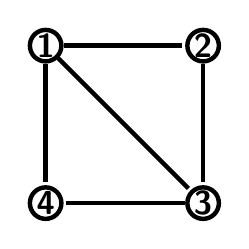
\begin{tikzpicture}[shorten >=1pt, auto, node distance=3cm, ultra thick,main node/.style={circle,draw,minimum size=.4cm,inner sep=0pt}]
\begin{scope}[every node/.style={font=\sffamily\large\bfseries}]
\node [main node](v1) at (0,0) {1};
\node [main node](v2) at (2,0) {2};
\node [main node](v3) at (2,-2) {3};
\node [main node](v4) at (0,-2) {4};
\end{scope}
\path 
	(v1) edge (v2)
    	 edge (v3)
         edge (v4)
    (v2) edge (v3)
    (v3) edge (v4)
    ;
\end{tikzpicture}
\end{figure}
$$\mathbb{P}=\begin{bmatrix}
0&\frac{1}{3}&\frac{1}{3}&\frac{1}{3}\\
\frac{1}{2}&0&\frac{1}{2}&0\\
\frac{1}{3}&\frac{1}{3}&0&\frac{1}{3}\\
\frac{1}{2}&0&\frac{1}{2}&0
\end{bmatrix}$$
\end{multicols}
\begin{enumerate}[label=\alph*)]
\item Wyznacz rozkład stacjonarny dla tego łańcucha.

\begin{align*}
&\bar{\pi}\mathbb{P}=\bar{\pi}\\
&\left[\pi _1, \pi _2,\pi _3,\pi _4\right]\begin{bmatrix}
0&\frac{1}{3}&\frac{1}{3}&\frac{1}{3}\\
\frac{1}{2}&0&\frac{1}{2}&0\\
\frac{1}{3}&\frac{1}{3}&0&\frac{1}{3}\\
\frac{1}{2}&0&\frac{1}{2}&0
\end{bmatrix}=\left[\pi _1, \pi _2,\pi _3,\pi _4\right]\\
&\left\{\begin{matrix}
\frac{1}{2}\pi _2 + \frac{1}{3}\pi _3+\frac{1}{2}\pi _4&=\pi _1\\
\frac{1}{3}\pi _1+\frac{1}{3}\pi _3&=\pi _2\\
\frac{1}{3}\pi _1+\frac{1}{2}\pi _2 +\frac{1}{2}\pi _4&=\pi _3\\
\frac{1}{3}\pi _1+\frac{1}{3}\pi _3&=\pi _4
\end{matrix}\right.\rightarrow \left\{\begin{matrix}
\pi _2 &= \frac{2}{3}\pi _1\\
\pi _3 &= \pi _1\\
\pi _4 &= \frac{2}{3}\pi _1
\end{matrix}\right.\\
&\frac{2}{3}x+\frac{2}{3}x+x+x=1\rightarrow \frac{10}{3}x=1\rightarrow x = \frac{3}{10}
\end{align*}
Rozkład stacjonarny ma postać: $\left[\frac{3}{10},\frac{1}{5},\frac{3}{10},\frac{1}{5}\right]$, 
\item Sprawdź, że łańcuch jest nieprzywiedlny i nieokresowy.

Łańcuch jest nieprzywiedlny, gdyż 
\begin{align*}
&\pi _{12}(1)=\pi _{13}(1)=\pi _{14}(1)=\frac{1}{3}\\
&\pi _{21}(1)=\pi _{23}(1)=\frac{1}{2} & pi _{24}(2)=\frac{1}{2}*\frac{1}{3}=\frac{1}{6}\\
&\pi _{31}(1)=\pi _{32}(1)=\pi _{34}(1)=\frac{1}{3}\\
&\pi _{41}(1)=\pi _{43}(1)=\frac{1}{2} & pi _{42}(2)=\frac{1}{2}*\frac{1}{3}=\frac{1}{6}\\
\end{align*}
więc z każdego dowolnego stanu do każdego innego stanu można przejść z prawdopodobieństwem $\pi _{ij}(t)>0$.

Przedstawiony łańcuch jest \textbf{nie} okresowy, gdyż
$$\mathsf{okr}(Ł)=1$$
\item Wyznacz przybliżone prawdopodobieństwo, że po 12345 krokach znajdziemy się z wierzchołku nr 1. Błąd przybliżenia nie jest istotny.

Zgodnie z wzorem z wykładu:
$$\bar{p}(0)\bar{\bar{\mathbb{P}}}^t\approx\bar{p}(t)\underset{r\rightarrow \infty}{\rightarrow} \bar{\pi}$$
to prawdopodobieństwo będzie wnosić (w przybliżeniu) $\frac{3}{10}$
\item Wyznacz przybliżone prawdopodobieństwo, że po 12345 krokach znajdziemy się z wierzchołku nr 1, a następnym kroku – w wierzchołku nr 2. Błąd przybliżenia nie jest istotny.

Kontynuując rozważania ww. wzoru:
$$\frac{3}{10}*\frac{1}{3}=\frac{3}{30}\approx\frac{1}{10}$$
\end{enumerate}

\paragraph{A9} Wyznacz rozkład stacjonarny dla klasycznego błądzenia po cyklu długości 12 z jedną przekątną. Przekątną w tym zadaniu można sobie wybrać samodzielnie.
\begin{figure}[H]
\centering
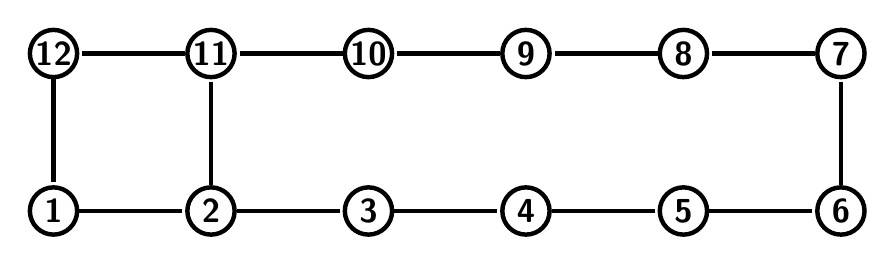
\begin{tikzpicture}[shorten >=1pt, auto, node distance=3cm, ultra thick,main node/.style={circle,draw,minimum size=.6cm,inner sep=0pt}]
\begin{scope}[every node/.style={font=\sffamily\large\bfseries}]
\node [main node](v1) at (0,0) {1};
\node [main node](v2) at (2,0) {2};
\node [main node](v3) at (4,0) {3};
\node [main node](v4) at (6,0) {4};
\node [main node](v5) at (8,0) {5};
\node [main node](v6) at (10,0) {6};
\node [main node](v7) at (10,2) {7};
\node [main node](v8) at (8,2) {8};
\node [main node](v9) at (6,2) {9};
\node [main node](v10) at (4,2) {10};
\node [main node](v11) at (2,2) {11};
\node [main node](v12) at (0,2) {12};
\end{scope}
\path 
	(v1) edge (v2)
    (v2) edge (v3)
    	 edge (v11)
    (v3) edge (v4)
    (v4) edge (v5)
    (v5) edge (v6)
    (v6) edge (v7)
    (v7) edge (v8)
    (v8) edge (v9)
    (v9) edge (v10)
    (v10) edge (v11)
    (v11) edge (v12)
    (v12) edge (v1)
    ;
\end{tikzpicture}
\end{figure}
\begin{align*}
&\pi _{i}=\frac{\deg (i)}{\sum \deg (i)}=\frac{\deg (i)}{2|E|}\\
&\pi _{1}=\pi _{3}=\pi _{4}=\pi _{5}=\pi _{6}=\pi _{7}=\pi _{8}=\pi _{9}=\pi _{10}=\pi _{12}=\frac{2}{26}=\frac{1}{13}\\
&\pi _{2}=\pi _{11}=\frac{3}{26}\\
&\bar{\pi}=\left[\frac{1}{13},\frac{3}{26},\frac{1}{13},\frac{1}{13},\frac{1}{13},\frac{1}{13},\frac{1}{13},\frac{1}{13},\frac{1}{13},\frac{1}{13},\frac{3}{26},\frac{1}{13}\right]
\end{align*}

\paragraph{A10} Oceń poprawność poniższych zdań. Odpowiedź ,,tak” należy poprzeć uzasadnieniem ogólnym, a Odpowiedź ,,nie” – kontrprzykładem (i uzasadnić poprawność kontrprzykładu). $\left[ p_{ij} \right]_{i,j\in S}$ oznacza, jak zwykle, macierz przejścia rozważanego łańcucha.
\begin{enumerate}[label=\alph*)]
\item Łańcuch jest nieprzywiedlny wtedy i tylko wtedy, gdy dla wszystkich jego stanów $i,\ j$ zachodzi $p_{ij} > 0$.

\textbf{TAK} (gdy $p_{i,j}$ oznacza $\pi_{i,j}(t)$ czytaj prawdopodobieństwo przejścia z $i$ do $j$ w $t$ krokach)
\begin{itemize}
\item[$\Rightarrow$] jeżeli łańcuch jest nieprzywiedlny to  da się ,,przejść'' z każdego jego stanu ($i$) do każdego innego stanu ($j$), więc prawdopodobieństwo przejścia z $i$ do $j$ jest większe od zera $\rightarrow$ $\pi _{i,j} > 0$
\item[$\Leftarrow$] gdy dla wszystkich stanów zachodzi $\pi _{i,j} > 0$, czyli  prawdopodobieństwo przejścia z $i$ do $j$ jest większe od zera to zgodnie z definicją \ref{def:NieprzywiedlnoscLM} (na stronie \pageref{def:NieprzywiedlnoscLM}) łańcuch jest nieprzywiedlny. 
\end{itemize}
\textbf{NIE} (gdy $p_{i,j}$ oznacza $\pi_{i,j}(1)$ czytaj prawdopodobieństwo przejścia z $i$ do $j$ w jednym kroku)
\begin{figure}[H]
\centering
\begin{tikzpicture}[shorten >=1pt, auto, node distance=3cm, ultra thick,main node/.style={circle,draw,minimum size=.6cm,inner sep=0pt}]
\begin{scope}[every node/.style={font=\sffamily\large\bfseries}]
\node [main node](v1) at (0,0) {1};
\node [main node](v2) at (2,0) {2};
\node [main node](v3) at (4,0) {3};
\node [main node](v4) at (4,2) {4};
\node [main node](v5) at (2,2) {5};
\node [main node](v6) at (0,2) {6};
\end{scope}
\path 
	(v1) edge [{triangle 45}-{triangle 45}] (v2)
    (v2) edge [{triangle 45}-{triangle 45}] (v3)
    (v3) edge [{triangle 45}-{triangle 45}] (v4)
    (v4) edge [{triangle 45}-{triangle 45}] (v5)
    (v5) edge [{triangle 45}-{triangle 45}] (v6)
    (v6) edge [{triangle 45}-{triangle 45}] (v1)
    ;
\end{tikzpicture}
\caption*{każda krawędź to prawdopodobieństwo $\sfrac{1}{2}$}
\end{figure}
Łańcuch jest nieprzywiedlny a $p_{1,5}=0$.

\item Jeżeli dla wszystkich stanów $i,\ j$ łańcucha Markowa zachodzi $p_{ij} = p_{ji}$, to łańcuch jest odwracalny.

\textbf{TAK} Łańcuch Markowa jest odwracalny, gdy istnieje wektor $\bar{a}$ i dla każdej pary $i,j$ zachodzi: $a_i\pi _{i,j}=a_j \pi _{j,i}$ w tym zadaniu wektor $\bar{\pi}$ będzie mieć postać: $\pi _i=\frac{1}{\sum _{s\in S}a_s}$, czytaj, każdy element wektora stacjonarnego ma taką samą wartość.
\item Jeżeli łańcuch jest odwracalny, to dla wszystkich jego stanów $i,\ j$ zachodzi $p_{ij} = p_{ji}$.

\textbf{NIE} Kontrprzykład: Graf $G=(V,E)$ ma postać:
\begin{multicols}{2}
\begin{figure}[H]
\centering
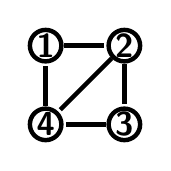
\begin{tikzpicture}[shorten >=1pt, auto, node distance=3cm, ultra thick,main node/.style={circle,draw,minimum size=.4cm,inner sep=0pt}]
\begin{scope}[every node/.style={font=\sffamily\large\bfseries}]
%\node (v0) at (-2,2) {START};
\node [main node](v1) at (0,0) {1};
\node [main node](v2) at (1,0) {2};
\node [main node](v3) at (1,-1) {3};
\node [main node](v4) at (0,-1) {4};
\end{scope}
\path 
%	(v0) edge [->] (v1)
	(v1) edge (v2)
    (v2) edge (v3)
    	 edge (v4)
    (v3) edge (v4)
    (v4) edge (v1)
    ;
\end{tikzpicture}
\end{figure}

\begin{figure}[H]
\centering
\begin{tikzpicture}[shorten >=1pt, auto, node distance=3cm, ultra thick,main node/.style={circle,draw,minimum size=.4cm,inner sep=0pt}]
\begin{scope}[every node/.style={font=\sffamily\large\bfseries}]
%\node (v0) at (-2,2) {START};
\node [main node](v1) at (0,0) {1};
\node [main node](v2) at (4,0) {2};
\node [main node](v3) at (4,-3) {3};
\node [main node](v4) at (0,-3) {4};
\end{scope}
\path 
%	(v0) edge [->] (v1)
	(v1) edge [->,bend left] node {$\sfrac{1}{2}$} (v2)
    	 edge [->] node {$\sfrac{1}{2}$} (v4)
    (v2) edge [->] node {$\sfrac{1}{3}$} (v1)
    	 edge [->,bend left] node {$\sfrac{1}{3}$} (v3)
         edge [->,bend left] node {$\sfrac{1}{3}$} (v4)
    (v3) edge [->] node {$\sfrac{1}{2}$} (v2)
    	 edge [->,bend left] node {$\sfrac{1}{2}$} (v4)
    (v4) edge [->,bend left] node {$\sfrac{1}{3}$} (v1)
    	 edge [->] node {$\sfrac{1}{3}$} (v2)
     	 edge [->] node {$\sfrac{1}{3}$} (v3)
    ;
\end{tikzpicture}
\end{figure}

$$\mathbb{P}=\begin{bmatrix}
0&\sfrac{1}{2}&0&\sfrac{1}{2}\\
\sfrac{1}{3}&0&\sfrac{1}{3}&\sfrac{1}{3}\\
\sfrac{1}{2}&0&0&\sfrac{1}{2}\\
\sfrac{1}{3}&\sfrac{1}{3}&\sfrac{1}{3}&0
\end{bmatrix}$$
\end{multicols}
\begin{align*}
&\left[\pi_1, \pi_2, \pi_3, \pi_4\right]\begin{bmatrix}
0&\sfrac{1}{2}&0&\sfrac{1}{2}\\
\sfrac{1}{3}&0&\sfrac{1}{3}&\sfrac{1}{3}\\
\sfrac{1}{2}&0&0&\sfrac{1}{2}\\
\sfrac{1}{3}&\sfrac{1}{3}&\sfrac{1}{3}&0
\end{bmatrix} = \left[\pi_1, \pi_2, \pi_3, \pi_4\right]\\
&\left[\pi_1, \pi_2, \pi_3, \pi_4\right] = \left[\frac{1}{5},\frac{3}{10},\frac{1}{5},\frac{3}{10}\right]\\
&\text{Przykład: }\\
&\pi _1\pi_{1,2}=\pi_2\pi_{21}\\
&\frac{1}{5}*\frac{1}{2}=\frac{3}{10}*\frac{1}{3}
\end{align*}


\item Jeżeli łańcuch o zbiorze stanów $S = \{1, 2\}$ jest nieokresowy i nieprzywiedlny, a jego rozkładem stacjonarnym jest $\left[\frac{1}{3}, \frac{2}{3}\right]$, to $p_{12}(n) \rightarrow \frac{2}{3}$ przy $n \rightarrow \infty$.

\textbf{TAK} zgodnie z twierdzeniem \ref{the:ergodycznoscLM2} (na stronie \pageref{the:ergodycznoscLM2}) zadanie można zapisać jako:
$$\lim _{n\rightarrow \infty} \pi _{1,2}(n)=\approx\frac{2}{3}$$

\item  Jeżeli łańcuch o zbiorze stanów $S = \{1,2\}$ jest nieokresowy i nieprzywiedlny, a jego rozkładem stacjonarnym jest $\left[ \frac{1}{3},\frac{2}{3}\right]$ to $p_{2,1}(n)\to\frac{2}{3}$ przy $n\to\infty$.

\textbf{NIE} kontrprzykład
\end{enumerate}

\subsection{Zadania domowe B}
\paragraph{B1} Obok podana jest macierz przejścia pewnego łańcucha Markowa.
$$\begin{bmatrix}
\frac{1}{5}&\frac{1}{5}&\frac{1}{5}&\frac{1}{5}&\frac{1}{5}\\
0&\frac{1}{2}&0&\frac{1}{2}&0\\
\frac{2}{3}&0&\frac{1}{6}&0&\frac{1}{6}\\
0&0&0&1&0\\
\frac{1}{4}&0&\frac{1}{4}&0&\frac{1}{2}
\end{bmatrix}$$
\begin{enumerate}[label=\alph*)]
\item Czy łańcuch jest nieprzywiedlny?
\item Czy posiada stany okresowe?
\item znajdź wszystkie rozkłady stacjonarne tego łańcucha.
\end{enumerate}

\paragraph{B2} Na podstawie podanej macierzy przejścia łańcucha Markowa znajdź przybliżone
prawdopodobieństwo, że po 2000 krokach łańcuch znajdzie się w stanie 3.
$$\begin{bmatrix}
\frac{1}{4}&\frac{1}{4}&\frac{1}{4}&\frac{1}{4}\\
0&0&\frac{3}{4}&\frac{1}{4}\\
\frac{1}{2}&0&0&\frac{1}{2}\\
1&0&0&0
\end{bmatrix}$$

\paragraph{B3} Pchła skacze po wierzchołkach ścieżki o 4 wierzchołkach. W każdym ruchu z prawdopodobieństwem $\frac{1}{2}$ zostaje na miejscu, a z prawdopodobieństwem $\frac{1}{2}$ zmienia Wierzchołek, przeskakując do wierzchołka przyległego, wybranego losowo w sposób jednostajny (czyli z jednakowym prawdopodobieństwem). Na początku Pchła z jednakowym prawdopodobieństwem znajduje się w dowolnym wierzchołku ścieżki. Jakie jest w przybliżeniu prawdopodobieństwo, że po 100tys. ruchów Pchła znajdzie się w pierwszym wierzchołku?

\paragraph{B4} Koń szachowy spaceruje po zwyczajnej szachownicy $8\times 8$. W każdym ruchu z pól, na które może skoczyć, wybiera losowo (z równym prawdopodobieństwem) jedno i na nie skacze. Jaki jest naturalny zbiór stanów dla łańcucha Markowa opisującego spacer konia? Czy łańcuch ów jest nieprzywiedlny? Czy ma stany okresowe?

\paragraph{B5} 50 zawodników gra w piłkę: co sekundę zawodnik posiadający piłkę rzuca ją do losowo wybranego innego zawodnika.
\begin{enumerate}[label=\alph*)]
\item Co wspólnego ma ta gra z błądzeniem losowym po grafach?
\item Oblicz (zdroworozsądkowo) prawdopodobieństwo, że piłka wróci do zawodnika rozpoczynającego grę w czasie krótszym niż 100s.
\end{enumerate}

\paragraph{B6} Rozważmy łańcuchy Markowa odpowiadające klasycznemu Błądzeniu na poniższych grafach. Sprawdź ich nieprzywiedlność, okresowość i wyznacz przykładowe rozkłady stacjonarne.
\begin{figure}[H]
\centering
\includegraphics[width=.9\textwidth]{img/9_B6}
\end{figure}

\paragraph{B7} Na łące przedzielonej niskim murkiem na część północną i południową bawi się $n$ świerszczy, o imionach $1, . . . , n$. Co minutę z prawdopodobieństwem $\sfrac{1}{4}$ zostają w miejscu, a z prawdopodobieństwem $\sfrac{3}{4}$ dokonuje się zmiana: losowo wybrany w sposób jednostajny świerszcz przeskakuje na drugą stronę. Budujemy dla zabawy świerszczy łańcuch Markowa, w którym Ważne jest ile świerszczy znajduje się na każdej stronie łąki oraz Ważne jest, które to świerszcze (mamy więc $2^n$ stanów).
\begin{enumerate}[label=\alph*)]
\item Czy łańcuch jest nieprzywiedlny?
\item Czy łańcuch jest okresowy?
\item Czy łańcuch jest odwracalny?
\item Oblicz przybliżone prawdopodobieństwo, że po 117345 minutach kostką wszystkie świerszcze znajdą się na północnej stronie łąki. Zwróć uwagę , że nie wiemy, po której stronie murku znajdują się świerszcze na początku zabawy.
\end{enumerate}

\paragraph{B8} Tasujemy talię $n$ ($n \geq 2$) kart w taki sposób: zaczynamy od dowolnego stosu, wybieramy losowo (z jednakowym prawdopodobieństwem) jedną
z $n$ kart i kładziemy ją na wierzch.
\begin{enumerate}[label=\alph*)]
\item Sprawdź, czy odpowiadający (w naturalny sposób) temu procesowi łańcuch Markowa jest odwracalny, dla trzech przypadków: $n = 2$, $n = 4$, $n = 52$.
\item Uzasadnij, że łańcuch jest nieokresowy i nieprzywiedlny.
\end{enumerate}

\paragraph{B9} Tasujemy ułożoną w stos talię 52 kart metodą losowych transpozycji: wybieramy losowo kolejno dwie (niekoniecznie różne) karty i zamieniamy je miejscami.
\begin{enumerate}[label=\alph*)]
\item Jaki jest przykładowy rozkład stacjonarny tak określonego łańcucha Markowa?
\item Czy łańcuch jest okresowy?
\item Czy łańcuch jest nieprzywiedlny?
\end{enumerate}

\paragraph{B10} Rozważamy błądzenie klasyczne na grafie $G$ o wierzchołkach $1, . . . , n$, który jest spójny i nie jest dwudzielny. Niech $\pi = [\pi_1, . . . , \pi_n]$ będzie rozkładem stacjonarnym dla tego błądzenia. oceń poprawność poniższych zdań. Odpowiedź należy poprzeć, jak zwykle, albo uzasadnieniem ogólnym, albo przykładem, albo kontrprzykładem.
\begin{enumerate}[label=\alph*)]
\item $p_{2,1}(t) \rightarrow \sfrac{\deg(1)}{2E(G)}$ przy $t\to \infty$.
\item Jeżeli Wierzchołek $2$ jest stopnia $5$, a $p_{2,1}(t) \rightarrow \frac{1}{40}$ przy $t\to \infty$, to $G$ ma dokładnie 100 krawędzi.
\item $p_{1,3}(t) \rightarrow \sfrac{\deg(1)}{2E(G)}$ przy $t\to \infty$.
\item Jeżeli Wierzchołek $3$ jest stopnia $4$, a $p_{2,3}(t) \rightarrow \frac{1}{100}$ przy $t\to \infty$, to $G$ ma więcej niż $100$ krawędzi.
\item Jeżeli $G$ jest grafem regularnym, to rozkład stacjonarny jest jednostajny.
\end{enumerate}

\paragraph{B11} oceń poprawność poniższych zdań. Odpowiedź należy poprzeć, jak zwykle, albo uzasadnieniem ogólnym, albo przykładem, albo kontrprzykładem.
\begin{enumerate}[label=\alph*)]
\item łańcuch jest nieprzywiedlny wtedy i tylko wtedy, gdy dla każdych jego stanów $i, j$ zachodzi $p_{ij}(1) > 0$.
\item Istnieje nieprzywiedlny i nieokresowy łańcuch Markowa, w którym dla każdego stanu $j$ zachodzi $p_{1,j} (n) \rightarrow 0$ przy $n \to \infty$.
\item Jeśli łańcuch Markowa posiada rozkład stacjonarny $[\pi_1, . . . , \pi_n]$, to dla każdego stanu $j$ zachodzi $p_{1,j} (n) \rightarrow 0$ przy $n \to \infty$.
\item każdy łańcuch Markowa ma dokładnie jeden rozkład stacjonarny.
\end{enumerate}

\subsection{Zadania}
\paragraph{Zad.1} Na podstawie podanej macierzy przejścia łańcucha Markowa
\begin{multicols}{3}
$$a)\ \begin{bmatrix}
\frac{1}{4}&\frac{1}{4}&\frac{1}{4}&\frac{1}{4}&0\\
0&0&\frac{1}{2}&\frac{1}{4}&\frac{1}{4}\\
0&0&0&1&0\\
0&0&0&1&0\\
0&0&0&0&1
\end{bmatrix}$$
$$b)\ \begin{bmatrix}
0&\sfrac{1}{2}&0&\sfrac{1}{2}\\
\sfrac{1}{3}&0&\sfrac{1}{3}&\sfrac{1}{3}\\
\sfrac{1}{2}&0&0&\sfrac{1}{2}\\
\sfrac{1}{3}&\sfrac{1}{3}&\sfrac{1}{3}&0
\end{bmatrix}$$
$$c)\ \begin{bmatrix}
0&\frac{1}{2}&0&\frac{1}{2}\\
\frac{1}{2}&0&\frac{1}{2}&0\\
0&\frac{1}{2}&0&\frac{1}{2}\\
\frac{1}{2}&0&\frac{1}{2}&0
\end{bmatrix}$$
\end{multicols}
\begin{itemize}
\item Sprawdź, czy łańcuch jest nieprzywiedlny.
\item Sprawdź, czy istnieją w nim stany okresowe.
\item wyznacz liczbę rozkładów stacjonarnych dla pierwszych dwóch łańcuchów.
\item znajdź przybliżone prawdopodobieństwo $p_{3,4}(2000)$ dla pierwszych dwóch łańcuchów.
\end{itemize}

\paragraph{Zad.2} Dany jest graf G bez wierzchołków izolowanych. Rozważmy klasyczne błądzenie na tym grafie.
\begin{enumerate}[label=\alph*)]
\item Po czym poznać, że łańcuch Markowa jest nieprzywiedlny?
\item Po czym poznać, że łańcuch Markowa jest nieokresowy?
\end{enumerate}

\paragraph{Zad.3} Rozważmy klasyczne błądzenie po cyklu na 4 wierzchołkach z przekątną, w którym Wierzchołek stopnia 3 ma numer 1. Jakie jest w przybliżeniu prawdopodobieństwo, że po 2000 krokach żeton znajdzie się
\begin{enumerate}[label=\alph*)]
\item w wierzchołku 1?
\item w jednym z wierzchołków stopnia 3?
\end{enumerate}

\paragraph{Zad.4} Rozważmy łańcuch Markowa z robaczkami z drugiego zadania poprzednich ćwiczeń (model z 4 stanami). Załóżmy, że na początku na trójkącie są dwa robaczki czerwone i jeden zielony. Jakie jest w przybliżeniu prawdopodobieństwo, że po 2000 sekundach nie wszystkie robaczki będą tego samego koloru?

\paragraph{Zad.5} Na łące przedzielonej niskim murkiem na część północną i południową bawią się trzy wesołe świerszcze: Jeden, Dwa i Trzy. Rzucają one kostką i kiedy wypadną na niej co najwyżej trzy oczka świerszcz o odpowiednim imieniu przeskakuje przez murek. Jeśli natomiast na kostce wypadną więcej niż trzy oczka, wszystkie świerszcze podskakują z radości, pozostając jednakże każdy po swojej stronie łąki. Budujemy dla zabawy świerszczy łańcuch Markowa, w którym Ważne jest ile świerszczy znajduje się na każdej stronie łąki, ale nie jest Ważne, które to świerszcze.
\begin{enumerate}[label=\alph*)]
\item Czy łańcuch jest odwracalny?
\item Oblicz przybliżone prawdopodobieństwo, że po 117345 rzutach kostką wszystkie świerszcze znajdą się na północnej stronie łąki. Zwróć uwagę , że nie wiemy, po której stronie murku znajdują się świerszcze na początku zabawy (pod tym względem rozbrykane świerszcze nie są tak przewidywalne jak ropuchy z zadania domowego).
\end{enumerate}

\paragraph{Zad.6} Tasujemy talię 3 kart w taki sposób: zaczynamy od dowolnego stosu, wybieramy losowo (z jednakowym prawdopodobieństwem) jedną z 3 kart i kładziemy ją na wierzch. Sprawdź, czy odpowiadający (w naturalny sposób) temu procesowi łańcuch Markowa jest odwracalny.
